\documentclass [11pt]{article}

\usepackage[utf8]{inputenc}
\usepackage[T1]{fontenc}
\usepackage[greek,portuguese]{babel}
\usepackage{graphicx}
\usepackage{minted}
\usepackage{fancyvrb}
\usepackage{xcolor}
\usepackage{listings}
\usepackage{hyperref}

\lstset{
  basicstyle=\ttfamily,
  columns=fullflexible,
  frame=single,
  breaklines=true,
  postbreak=\mbox{\textcolor{red}{$\hookrightarrow$}\space},
}

\renewcommand{\lstlistingname}{Algoritmo}

\title{Trabalho Prático II}
\author{Universidade Federal de Minas Gerais \\ Departamento de Ciência da Computação \\ Compiladores I \\ \\ João Francisco B. S. Martins,  Pedro D. V. Chaves \\ \texttt{\{joaofbsm, pedrodallav\}@dcc.ufmg.br}}

\begin{document}
\maketitle

\section{Introdução}

Um compilador é composto por duas partes principais: o \textit{front end} e o \textit{back end}. O \textit{front end} analisa o código fonte a fim de construir uma representação interna do programa, chamada de representação intermediária. Para tal ele se utiliza de uma estrutura de dados chamada tabela de símbolos, a qual será passada adiante junto com a representação gerada. Já o \textit{back end} trata da construção do programa objeto a partir da representação intermediária e da tabela de símbolos, realizando otimizações no código, quando possível.

O trabalho em questão tem como objetivo implementar o \textit{front end} de um compilador, cujas fases estão destacadas na Figura \ref{fig:front_end}, para a linguagem \textbf{SmallL}. Essa linguagem é descrita pela gramática apresentada na Figura \ref{fig:grammar}. Para codificação dos componentes do compilador se utilizou a linguagem de programação \textbf{Java} (\textit{v.8}). 

O trabalho foi desenvolvido utilizando a ferramenta de versionamento Git juntamente com a plataforma de desenvolvimento remoto GitHub. O repositório do projeto contém não só o código fonte, mas também os scripts auxiliares desenvolvidos e os arquivos de teste, podendo ser acessado no endereço \url{https://github.com/joaofbsm/smallL}.

\begin{figure}[H]
 	\centering
	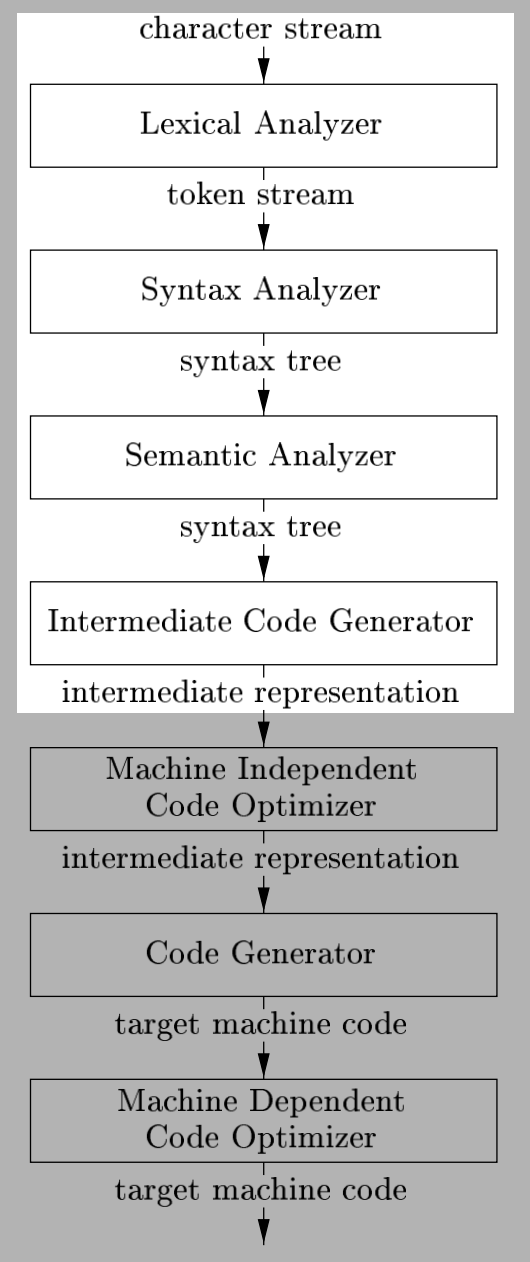
\includegraphics[width=6cm,keepaspectratio]{imgs/front_end.png}
	\caption{Componentes do \textit{front end} de um compilador (destacados em branco)}.
	\label{fig:front_end}
\end{figure}

\begin{figure}[H]
 	\centering
	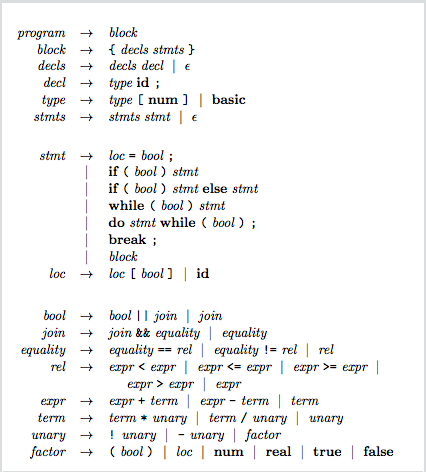
\includegraphics[width=1\textwidth]{imgs/grammar.png}
	\caption{Gramática inicial que descreve a linguagem \textbf{SmallL}}.
	\label{fig:grammar}
\end{figure}
\section{Desenvolvimento}

\subsection{Visão Geral}

O \textbf{tradutor} em questão teve sua implementação feita através da linguagem \textbf{Python} pela maior facilidade presente para manipulação de cadeias de caracteres (passo essencial para a tradução). Além disso, Python foi usada para tornar a comunicação com a ferramenta \textbf{Krakatau} mais fácil e eficiente.

O \textit{front-end} implementado no trabalho anterior tem como saída um código intermediário que tem por base 7 tipos de operações possíveis:

\begin{itemize}
\item \textbf{atribuição direta}: \texttt{x = y}
\item \textbf{atribuição com expressão aritmética}: \texttt{x = y arith\_op z}
\item \textbf{atribuição para posição de vetor}: \texttt{x[p] = y}
\item \textbf{atribuição de posição de vetor}: \texttt{x = y[p]}
\item \textbf{if com comparação}: \texttt{if x logic\_op y goto L}
\item \textbf{iffalse com comparação}: \texttt{iffalse x logic\_op y goto L}
\item \textbf{desvio}: \texttt{goto L}
\end{itemize}

A partir dos formatos de operações descritos acima, foi possível desenvolver um \textbf{tradutor} que indentificasse cada tipo de formato no arquivo de saída do gerador de código intermediário e gerasse código na sintaxe \textbf{Jasmin}, que por sua vez seria passado para o \textit{assembler} do \textbf{Krakatau} para gerar \textit{bytecodes} binários.


\subsection{Implementação}

O \textbf{tradutor} é implementado através dos 4 arquivos abaixo (além da integração com o \textbf{Krakatau}):

\begin{itemize}
\item \texttt{translator.py}: parseia e traduz o arquivo de código intermediário para \textit{bytecodes} Java utilizando sintaxe \textbf{Jasmin}. 
\item \texttt{opbuilder.py}: constrói operações baseadas na sintaxe de \textit{bytecodes} \textbf{Jasmin}.
\item \texttt{operation.py}: classe auxiliar para estruturar a representação de uma \textbf{operação}.
\item \texttt{variable.py}: classe auxiliar para estruturar a representação de uma \textbf{variável}.
\end{itemize}

O arquivo \texttt{translator.py} parseia o arquivo de entrada, gerando dicionários para os \textit{labels} (um dicionário para guardar os diferentes \textit{labels} e suas respectivas linhas e outro para guardar referências para \textit{labels} já existentes).

O bytecode não permite que uma mesma linha possua mais de um \textit{label}, como pode ocorrer no código intermediário. Sendo assim, uma forma de criar equivalências entre \textit{labels} foi implementada utilizando um dicionário, que é preenchido nessa primeira passada sob o arquivo.

Uma vez identificados os \textit{labels}, são geradas uma ou mais operações equivalentes na sintaxe \textbf{Jasmin}. Isso é feito através do módulo \texttt{opbuilder.py}, que mapeia cada uma dos formatos das quádruplas elucidadas acima para uma operação equivalente em \textbf{Jasmin}.

\subsection{Operações em bytecode}

A seguir será mostrado como cada tipo de operação que pode estar presente no código intermediário é mapeada para uma possível sequência de códigos na sintaxe \textbf{Jasmin}.

\subsubsection{Atribuição direta: \texttt{x = y} }

Uma atribuição simples é baseada em duas ações: carregar um operando (\texttt{y}) da memória (checando a tabela de símbolos) e salvar esse valor no operando do lado esquerdo \texttt{x}. No código abaixo, os valores de \texttt{x} e \texttt{y} já haviam sido inicializados (com valores nos endereços 1 e 3, respectivamente)


\begin{lstlisting}[caption=Operação de atribuição em código intermediário.]
L1:	x = y
\end{lstlisting}


\begin{lstlisting}[caption=Operação de atribuição simples em Jasmin.]
L1:		dload 3
      dstore 1
\end{lstlisting}

\subsubsection{Atribuição com expressão aritmética: \texttt{x = y arith\_op z} }

Uma atribuição com expressão é baseada em 3 operandos (\texttt{x} (op1), \texttt{y} (op2) e \texttt{z} (op3) ) e um operador aritmético (\texttt{arith\_op}). A atribuição segue as seguintes ações: primeiro carregam-se os operandos 2 e 3 da memória. Depois, os operandos 2 e 3 são somados através do comando \texttt{dload} (ações baseadas em pilha). Por final, o valor somado é salvo no operando 1 (os operandos 1, 2 e 3 estavam salvos nos endereços 1, 3 e 5, respectivamente). A sequência de passos pode ser vista no código abaixo, podendo-se substituir os operandos 2 e 3 por constantes caso algum desses fosse uma constante (utilizando o comando \texttt{ldc2\_w 1.0}, por exemplo).


\begin{lstlisting}[caption=Operação de atribuição com expressão aritmética em código intermediário.]
L2:	x = y + z
\end{lstlisting}


\begin{lstlisting}[caption=Operação de atribuição com expressão aritmética em Jasmin.]
L2:	     dload 3
     dload 5
     dadd
     dstore 1
\end{lstlisting}


\subsubsection{Atribuição para posição de vetor: \texttt{a[x] = z} }

Uma atribuição para posição de vetor requer uma sequência maior de passos. Explicaremos o passo a passo de cada trecho de código presente no Código 6:

\begin{lstlisting}
dload 1
ldc2_w 8.0
dmul
dstore 7
\end{lstlisting}

A JVM não requer a multiplicação do índice por 8 nos vetores, ou seja, sempre que é recebida uma variável que vai ser o índice de um array, ela por \textit{default} já é multiplicada por 8.

O código imediatamente acima carrega o valor que vai ser o índice (salvo no endereço 1), carrega a constante 8 na pilha e multiplica. Os próximos passos são indicados abaixo:

\begin{lstlisting}
sipush 1000
newarray double
astore 9
\end{lstlisting}

Cria um \textit{array} de double de 1000 posições (por \textit{default}) e salva na memória na posição 9.

\begin{lstlisting}
dload 7
ldc2_w 8.0
ddiv
dstore 7
\end{lstlisting}

O tradutor identifica que o endereço 7 vai ser usado como o índice do array, carrega esse endereço na pilha e também carrega a constante 8. Após isso, divide ambos e salva novamente no endereço 7.

\begin{lstlisting}
aload 9
dload 7
d2i
dload 5
dastore
\end{lstlisting}

Por último, carrega o ponteiro do \textit{array} (endereço 9) e  carrega a variável temporária que representa o índice (endereço 7). Pega o valor mais alto na pilha e converte de \texttt{double} para \texttt{int} (comando \texttt{d2i}), para que indexação seja possível. Finaliza carregando o valor a ser atribuído para a posição do vetor e salva esse valor na posição. 

Abaixo podemos ver a sequência de passos completa.


\begin{lstlisting}[caption=Atribuição para posição de vetor em código intermediário.]
L3:	t1 = x * 8
     a [ t1 ] = z
\end{lstlisting}

\begin{lstlisting}[caption=Atribuição para posição de vetor em Jasmin.]
L3:    dload 1
     ldc2_w 8.0
     dmul
     dstore 7
     sipush 1000
     newarray double
     astore 9
     dload 7
     ldc2_w 8.0
     ddiv
     dstore 7
     aload 9
     dload 7
     d2i
     dload 5
     dastore
\end{lstlisting}


\subsubsection{Atribuição de posição de vetor: \texttt{y = a[p]} }

A atribuição de posição de vetor segue um raciocínio bem semelhante ao elucidado anteriormente na atribuição para posição de vetor, mudando apenas a ordem de alguns \textit{loads} e \textit{stores}. No exemplo abaixo, o valor de \texttt{p} é uma constante (igual a 1, indicando o índice 1).


\begin{lstlisting}[caption=Atribuição de variável utilizando valor na posição de vetor em código intermediário.]
L4:	t3 = 1 * 8
  y = a [ t3 ]
\end{lstlisting}

\begin{lstlisting}[caption=Atribuição de variável utilizando valor na posição de vetor em Jasmin.]
L4: 	ldc2_w 1.0
    ldc2_w 8.0
    dmul
    dstore 13
    dload 13
    ldc2_w 8.0
    ddiv
    dstore 13
    aload 9
    dload 13
    d2i
    daload
  dstore 3
\end{lstlisting}


\subsubsection{Condicional comparativo: \texttt{if/iffalse x logic\_op y goto L} }

A comparação iffalse é feita da seguinte forma: primeiro são carregados os operandos (x e y) a serem comparados (na pilha) e em seguida o comando \texttt{dcmpl} compara os dois números, retornando como resultado 0 se forem iguais, 1 se y maior que x e -1 caso contrário. O último comando (\texttt{iflt}) verifica o resultado e, se x menor que y, desvia para L2.

\begin{lstlisting}[caption=iffalse com comparação em código intermediário]
L6:	iffalse x >= y goto L2
\end{lstlisting}

\begin{lstlisting}[caption=iffalse com comparação em Jasmin]
L6: dload 1
     dload 3
     dcmpl
     iflt L2
\end{lstlisting}

A diferença de \texttt{iffalse} e \texttt{if} é baseada no fato de iffalse ser utilizado com operador de maior ou igual (\texttt{>=}) e if ser utilizado com operador de menor (\texttt{<}).

Com isso, uma tradução de uma operação com if, geraria a seguinte sequência:
\begin{lstlisting}[caption=if com comparação em Jasmin]
L6: dload 1
     dload 3
     dcmpl
     ifgt L2
\end{lstlisting}

Ou seja, com a lógica "inversa" do iffalse, pois utiliza o comando \texttt{ifgt}, verificando o resultado de \texttt{dcmpl} de forma invertida.

\subsubsection{Desvio: \texttt{goto L}}
O comando de desvio funciona da mesma forma (e com a mesma sintaxe) em ambos os códigos (intermediário e na sintaxe Jasmin).


\section{Código e Utilização}

Por ser muito extenso, preferimos não descrever todo o código do \textbf{tradutor} neste documento, disponibilizando-o no repositório mencionado na seção de introdução.

Para obter o código, basta clonar o repositório utilizando o comando:

\begin{lstlisting}
git clone https://github.com/joaofbsm/smallL.git
\end{lstlisting}

ou baixar o \texttt{.zip} disponibilizado ao clicar em \textbf{"Clone or download"} e depois em \textbf{"Download ZIP"} (na página do repositório).

Caso tenha optado pela segunda opção, basta descompactar e entrar na pasta descompactada.

\subsection{Traduzindo}
Para facilitar a utilização do \textbf{tradutor} foram criados dois scripts \textit{bash} que condensam as tarefas de compilar o código do \textit{front-end}  e executar o \textit{front-end} (necessário para geração das quadruplas).

\begin{itemize}
\item \texttt{compile.sh}: responsável por compilar as classes Java necessárias para o funcionamento do \textit{front end}.
\item \texttt{execute.sh}: reponsável por testar todas as entradas de teste (código na linguagem \textbf{SmallL}) disponibilizadas no diretório \texttt{tests}.
\end{itemize}

Para traduzir os códigos intermediários gerados, basta executar o script \texttt{translate.sh} (após ter executado os dois scripts citados acima).

Para criar um caso de teste, basta adicionar um arquivo \texttt{.txt}, contendo o teste desejado (em linguagem SmallL), no diretório \texttt{tests} presente no diretório raiz do \textit{front-end}.

Caso deseje rodar um teste em específico, cuja entrada já está em formato de código intermediário, basta rodar:

\begin{lstlisting}
// mude para o diretorio raiz do front end
cd /caminho_para_diretorio_raiz/smallL
cd code/translator
python3 translator.py codigo_intermediario
\end{lstlisting}

Tal comando produzirá na saída padrão o código traduzido na sintaxe Jasmin. Para rodar a sequência de scripts completa, siga os seguintes passos:

\begin{lstlisting}
// mude para o diretorio raiz do front end
cd /caminho_para_diretorio_raiz/smallL
// compila
./compile.sh
// executa front-end
./execute.sh
// traduz codigo intermediario
./translate.sh
\end{lstlisting}

A saída dos testes se encontra na pasta \texttt{outputs}. Os \texttt{.txt} gerados são referentes ao código intermediário gerado pelo \textit{front-end}. Dentro do diretório \texttt{outputs} há uma pasta denominada \texttt{translated} que contém os códigos em Jasmin (\texttt{.j}) gerados pelo \textbf{tradutor} e os binários gerados pelo \textbf{Krakatau} (arquivos \texttt{.class} dentro das pastas \texttt{nome\_teste-bin/}), a partir dos códigos gerados pelo tradutor.

Para uma melhor formatação da saída, é aconselhável rodar o \texttt{disassembler} do \textbf{Krakatau} nos arquivos \texttt{.class} gerados. Para tal, rode a seguinte linha de comando:

\begin{lstlisting}
\\ entre no diretorio com a saida binaria
cd caminho_para_smallL/outputs/translated/nome_teste-bin/
\\ rode o disassembler
python2.7 ../../../tools/Krakatau/disassemble.py Main.class
\end{lstlisting}

Tal comando produzirá um arquivo \texttt{Main.j} em sintaxe Jasmin, contendo o código produzido pelo tradutor em uma formatação mais clara e organizada.
\section{Testes}

A seguir são apresentados alguns testes que tentam englobar todas as possíveis instruções geradas em sintaxe Jasmin. A sequência de arquivos para cada teste é a seguinte:

\begin{enumerate}
\item arquivo em linguagem \textbf{SmallL}
\item arquivo com código intermediário gerado a partir de 1.
\item arquivo com código traduzido a partir de 2.
\end{enumerate}


\subsection{Teste 1}

\begin{lstlisting}[caption=Arquivo para o teste 1 em linguagem SmallL]
{
    int x; int y; int z; float d; float e; float[3] a;
    
    x = 1;
    y = 10;
    z = 5;
    
    x = y;
    x = y + z;

    a[x] = z;
    a[2] = 1.5;

    y = a[1];

    if( x >= y ) x = 1;
}
\end{lstlisting}

\begin{lstlisting}[caption=Arquivo com código intermediário para o teste 1 produzido pelo front-end]
L1:	x = 1
L3:	y = 10
L4:	z = 5
L5:	x = y
L6:	x = y + z
L7:	t1 = x * 8
    a [ t1 ] = z
L8:	t2 = 2 * 8
    a [ t2 ] = 1.5
L9:	t3 = 1 * 8
    y = a [ t3 ]
L10:	iffalse x >= y goto L2
L11:	x = 1
L2:
\end{lstlisting}

\begin{lstlisting}[caption=\textbf{Código em sintaxe Jasmin para o teste 1 produzido pelo tradutor implementado}]
.version 50 0 
.class public super Main 
.super java/lang/Object 

.method public <init> : ()V 
	.code stack 1 locals 1 
L0:		aload_0 
L1:		invokespecial Method java/lang/Object <init> ()V 
L4:		return 
L5:     
	.end code 
.end method 

.method public static main : ([Ljava/lang/String;)V
	.code stack 4 locals 50

L1:											 ldc2_w 1.0
		dstore 1
L3:											 ldc2_w 10.0
		dstore 3
L4:											 ldc2_w 5.0
		dstore 5
L5:											 dload 3
		dstore 1
L6: 	dload 3
		dload 5
		dadd
		dstore 1
L7:											 dload 1
		ldc2_w 8.0
		dmul
		dstore 7
		sipush 1000
		newarray double
		astore 9
		dload 7
		ldc2_w 8.0
		ddiv
		dstore 7
		aload 9
		dload 7
		d2i
		dload 5
		dastore
L8:											 ldc2_w 2.0
		ldc2_w 8.0
		dmul
		dstore 11
		dload 11
		ldc2_w 8.0
		ddiv
		dstore 11
		aload 9
		dload 11
		d2i
		ldc2_w 1.5
		dastore
L9:											 ldc2_w 1.0
		ldc2_w 8.0
		dmul
		dstore 13
		dload 13
		ldc2_w 8.0
		ddiv
		dstore 13
		aload 9
		dload 13
		d2i
		daload
		dstore 3
L10:											 dload 1
		dload 3
		dcmpl
		iflt L2
L11:											 ldc2_w 1.0
		dstore 1
L2:											 return
	.end code 
.end method 
.sourcefile 'Main.java' 
.end class

\end{lstlisting}


\subsection{Teste 2}

\begin{lstlisting}[caption=Arquivo do teste 2 em linguagem SmallL]
{
    int i; int j; float v; float x; float[3] a;
    i = 1;
    j = 10;
    v = 2;
    x = 6;
    a[0] = 1;
    a[1] = 2;
    a[2] = 3;

    while( true ) {
        do i = i+1; while( a[i] < v);
        do j = j-1; while( a[j] > v);
        if( i >= j ) break;
        x = a[i]; a[i] = a[j]; a[j] = x;
    }
}
\end{lstlisting}

\begin{lstlisting}[caption=Arquivo com código intermediário para o teste 2 produzido pelo front-end]
L1:	i = 1
L3:	j = 10
L4:	v = 2
L5:	x = 6
L6:	t1 = 0 * 8
    a [ t1 ] = 1
L7:	t2 = 1 * 8
    a [ t2 ] = 2
L8:	t3 = 2 * 8
    a [ t3 ] = 3
L9:L10:	i = i + 1
L12:	t4 = i * 8
      t5 = a [ t4 ]
      if t5 < v goto L10
L11:	j = j - 1
L14:	t6 = j * 8
      t7 = a [ t6 ]
      if t7 > v goto L11
L13:	iffalse i >= j goto L15
L16:	goto L2
L15:	t8 = i * 8
      x = a [ t8 ]
L17:	t9 = i * 8
      t10 = j * 8
      t11 = a [ t10 ]
      a [ t9 ] = t11
L18:	t12 = j * 8
      a [ t12 ] = x
      goto L9
L2:

\end{lstlisting}

\begin{lstlisting}[caption=\textbf{Código para o teste 2 em sintaxe Jasmin produzido pelo tradutor implementado}]
.version 50 0 
.class public super Main 
.super java/lang/Object 

.method public <init> : ()V 
	.code stack 1 locals 1 
L0:		aload_0 
L1:		invokespecial Method java/lang/Object <init> ()V 
L4:		return 
L5:     
	.end code 
.end method 

.method public static main : ([Ljava/lang/String;)V
	.code stack 4 locals 50

L1:												 ldc2_w 1.0
		dstore 1
L3:												 ldc2_w 10.0
		dstore 3
L4:												 ldc2_w 2.0
		dstore 5
L5:												 ldc2_w 6.0
		dstore 7
L6:												 ldc2_w 0.0
		ldc2_w 8.0
		dmul
		dstore 9
		sipush 1000
		newarray double
		astore 11
		dload 9
		ldc2_w 8.0
		ddiv
		dstore 9
		aload 11
		dload 9
		d2i
		ldc2_w 1.0
		dastore
L7:												 ldc2_w 1.0
		ldc2_w 8.0
		dmul
		dstore 13
		dload 13
		ldc2_w 8.0
		ddiv
		dstore 13
		aload 11
		dload 13
		d2i
		ldc2_w 2.0
		dastore
L8:												 ldc2_w 2.0
		ldc2_w 8.0
		dmul
		dstore 15
		dload 15
		ldc2_w 8.0
		ddiv
		dstore 15
		aload 11
		dload 15
		d2i
		ldc2_w 3.0
		dastore
L9:												 dload 1
		ldc2_w 1.0
		dadd
		dstore 1
L12:											 dload 1
		ldc2_w 8.0
		dmul
		dstore 17
		dload 17
		ldc2_w 8.0
		ddiv
		dstore 17
		aload 11
		dload 17
		d2i
		daload
		dstore 19
		dload 19
		dload 5
		dcmpg
		iflt L9
L11:											 dload 3
		ldc2_w 1.0
		dsub
		dstore 3
L14:											 dload 3
		ldc2_w 8.0
		dmul
		dstore 21
		dload 21
		ldc2_w 8.0
		ddiv
		dstore 21
		aload 11
		dload 21
		d2i
		daload
		dstore 23
		dload 23
		dload 5
		dcmpl
		ifgt L11
L13:											 dload 1
		dload 3
		dcmpl
		iflt L15
L16:											 goto L2
L15:											 dload 1
		ldc2_w 8.0
		dmul
		dstore 25
		dload 25
		ldc2_w 8.0
		ddiv
		dstore 25
		aload 11
		dload 25
		d2i
		daload
		dstore 7
L17:											 dload 1
		ldc2_w 8.0
		dmul
		dstore 27
		dload 3
		ldc2_w 8.0
		dmul
		dstore 29
		dload 29
		ldc2_w 8.0
		ddiv
		dstore 29
		aload 11
		dload 29
		d2i
		daload
		dstore 31
		dload 27
		ldc2_w 8.0
		ddiv
		dstore 27
		aload 11
		dload 27
		d2i
		dload 31
		dastore
L18:											 dload 3
		ldc2_w 8.0
		dmul
		dstore 33
		dload 33
		ldc2_w 8.0
		ddiv
		dstore 33
		aload 11
		dload 33
		d2i
		dload 7
		dastore
		goto L9
L2:											 return
	.end code 
.end method 
.sourcefile 'Main.java' 
.end class
\end{lstlisting}


\section{Conclusão}

A partir do desenvolvimento dos trabalhos anteriores e da finalização por meio deste, foi possível compreender como funciona um compilador em todas as possíveis partes internas.

Conseguimos implementar tanto o \textit{front-end} \cite{aho2007compilers} quanto uma versão simples do \textit{back-end}(tradutor) do compilador de forma prática e eficaz, para uma gramática relativamente parecida com a de uma linguagem de programação amplamente utilizada (C ou Java).

Pudemos aprender sobre o funcionamento das análises léxica e sintática, geração de código intermediário e sobre a geração de \textit{bytecodes} via tradução, a partir do código intermediário.

Por fim, foi possível integrar todas as partes desenvolvidas com sucesso e também disponibilizar o código para qualquer pessoas que deseja utilizar essa implementação.

\bibliographystyle{IEEEannot}
\bibliography{annot}
\end{document}